%%%%%%%%%%%%%%%%%%%%%%%%%%%%%%%%%%%%%%%%%%%%%%%%%%%%%%%%%%%%%%%%%%%%
%%%% LVF_iclr2015_v1.tex file
%%%% Authors: Michael Giering, Kishore Reddy, Vivek Venugopalan
%%%% adapted from iclr2015.tex
%%%% v1 12-15-2014 13:35:11
%%%%%%%%%%%%%%%%%%%%%%%%%%%%%%%%%%%%%%%%%%%%%%%%%%%%%%%%%%%%%%%%%%%

\documentclass{article}
\usepackage{iclr2015,times} 
\usepackage{hyperref}
\usepackage{url}
\usepackage[pdftex]{graphicx}


\title{Multi-modal Sensor Registration for Vehicle Perception via Deep Neural Networks}

\author{Michael Giering, Kishore Reddy, Vivek Venugopalan\\
Decision Support \& Machine Intelligence Group \\
United Technologies Research Center\\
E. Hartford, CT 06060, USA \\
Email: {gierinmj, kkreddy, venugov}@utrc.utc.com}


\newcommand{\fix}{\marginpar{FIX}}
\newcommand{\new}{\marginpar{NEW}}

\iclrconference
\begin{document}


\maketitle

\begin{abstract}
When performing multi-modal fusion to perform an analytic task, spatio-temporal registration of the incoming signals is often a prerequisit to analyzing the fused data and critical to the stability of the analysis. Lidar-Video systems like on those many driverless cars are a common example of where keeping the Lidar and video channels registered to common physical features is important. We develop a deep learning method that takes multiple channels of heterogeneous data to detect the misalignment of the Lidar-video inputs. A number of variations were tested on the Ford LV driving test data set with minimal tuning of the deep conv nets parameters. 

\end{abstract}

\section{Motivation}
% please include other motivations
Navigation and situational awareness of optionally manned vehicles requires the integration of multiple sensing modalities such as LIDAR and video, but could just as easily be extended to other modalities including Radar, SWIR and GPS. Spatio-temporal registration of information from multi-modal sensors is technically challenging in its own right. For many tasks such as pedestrian and object detection tasks that make use of multiple sensors, decision support methods rest on the assumption of proper registration. Most approaches [][] in LIDAR-video for instance, build separate vision and lidar feature extraction methods and then try to identify common anchor points in both. Generating a single feature set on Lidar, Video and optical flow, enables the system to to capture mutual information among modalities more efficiently. The ability to dynamically register information from the available data channels for perception related tasks can alleviate the need for anchor points \emph{between} sensor modalities. We see auto-registration as a prerequisit need for operating on multi-modal information with confidence.

%better fusion
Deep neural networks lend themselves in a seamless manner for data fusion on time series data. It has been shown [Ng multimodal] for some problems that features generated on the fused information [] can provide insight that neither input alone can. In effect the ML version of, "the whole is greater than the sum of it's parts". 

%speed constraints
Speed constraints of real time navigation also constrain model selection. The trained nnets easily run within the real-time constraints of common frame rates and lidar data collection.

%Applied research perspective
From an applied research perspective, it is possible to create such systems with far less overhead. The need for domain experts and hand-crafted feature design are lessened, thereby allowing more rapid prototyping and testing. 

%%probably in next steps
The generalization of autoregistration across multiple assets is clearly a path to be explored. 

%%dynamics
By including optical flow as input channels, we imbue the nnet with information on the dynamics observed across time steps. 

\section{Previous Work} % (fold)
\label{sec:previous_work}
Need some references to define the state of the art 

% section previous_work (end)



\section{Problem Statement} % (fold)
\label{sec:problem_statement}
% need detailed description and citation regarding the ford data set
% need greater clarity on the optical flow method used.

Being able to detect and correct the misalignment (registration, calibration) among sensors of the same or different kinds is critical when operating on the fused information emanating from them. For this work DCNN's were implemented for the detection of small spatial misalignments in Lidar and Video frames. The data was collected from a driverless car was chosen as the multi-modal fusion test case. LV is a common combination for providing perception capabilities to many types of ground and airborne platforms including driverless cars [google, ford]. 

The FORD LIDAR-Video dataset \cite{Pandey2011Ford-campu} is collected by an autonomous Ford F-250 vehicle integrated with the following perception and navigation sensors:
\begin{itemize}
    \item Velodyne HDL-64E LIDAR with two blocks of lasers spinning at 10 Hz and a maximum range of 120m.
\end{itemize}


\subsection{Ford LIDAR-Video Dataset and Experimental Setup} % (fold)
\label{sub:ford_lidar_video_dataset_and_experimental_setup}

\textbf{ Kishore -Detailed description of the ford data set [], our test and training and the justifications for it. framerate. 
Vivek - a brief description of the hardware used. }

% Ford Dataset
%% image the ford data collection system and camera views
\begin{figure}[htbp]
    \centering
        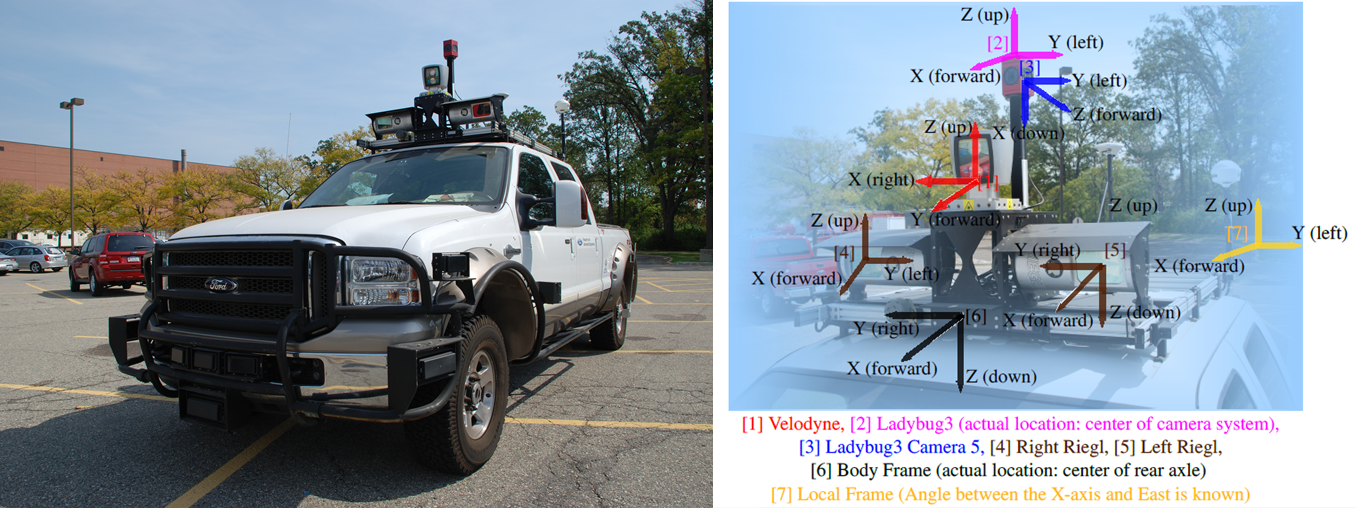
\includegraphics[scale=0.45]{Figures/ford-truck-sensors.png}
    \caption{Left: The modified Ford F-250 pickup truck \cite{Pandey2011Ford-campu}. Right: Relative position of the sensors with respect to the body frame \cite{Pandey2011Ford-campu}.}
    \label{fig:ford-truck-sensors}
\end{figure}

Ford Campus Vision and Lidar dataset \citep{Pandey2011Ford-campu} (Ford-VL) is a publicly available dataset collected by an autonomous ground vehicle mounted with multiple sensors shown in Figure~\ref{fig:ford-truck-sensors}. In this work we used time-registered Velodyne 3D-lidar scanner (Lidar) and Point Grey Ladybug3 omnidirectional camera(Video) data collected while driving in a loop in the downtown Dearborn Michigan. Velodyne sensor has a range of 120 m with the lidar spinning at 10 Hz. Video is captured at 8 fps (1600x600 resolution) using array of six 2-Megapixel cameras to collect video from 80\% of sphere.  

%% image of Ford Data set marked with Testing and Training
\begin{figure}[htbp]
    \centering
        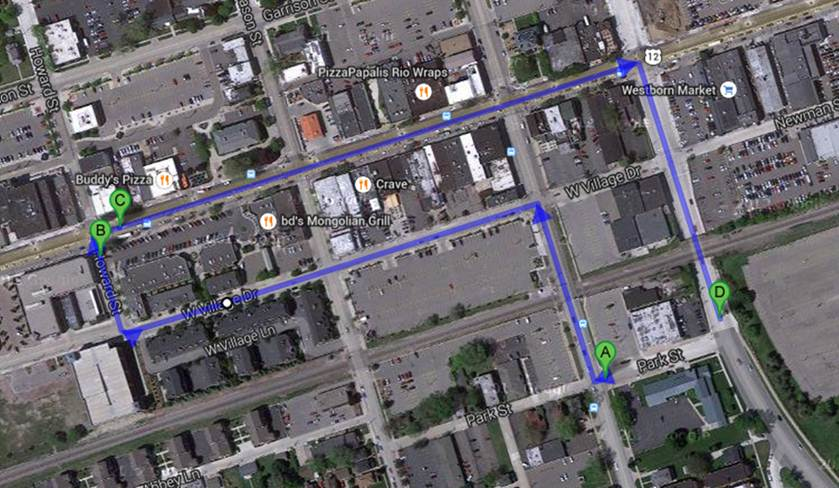
\includegraphics[scale=0.35]{Figures/ford_train_test_track.jpg}
    \caption{Training (A to B) and testing (C to D) tracks in the downtown Dearborn Michigan.}
    \label{fig:ford_train_test_track}
\end{figure}

As shown in Figure~\ref{fig:ford_train_test_track}, we divided the data set into training and testing sections A to B and C to D respectively. They were chosen in a manner that minimizes the likelihood of contamination between training and testing. Because of this, the direction of the lighting is source is never the same in the testing and training sets. If our methods are generalizable, they should be able to overcome this bias in the data.   

\begin{figure}[htbp]
    \centering
        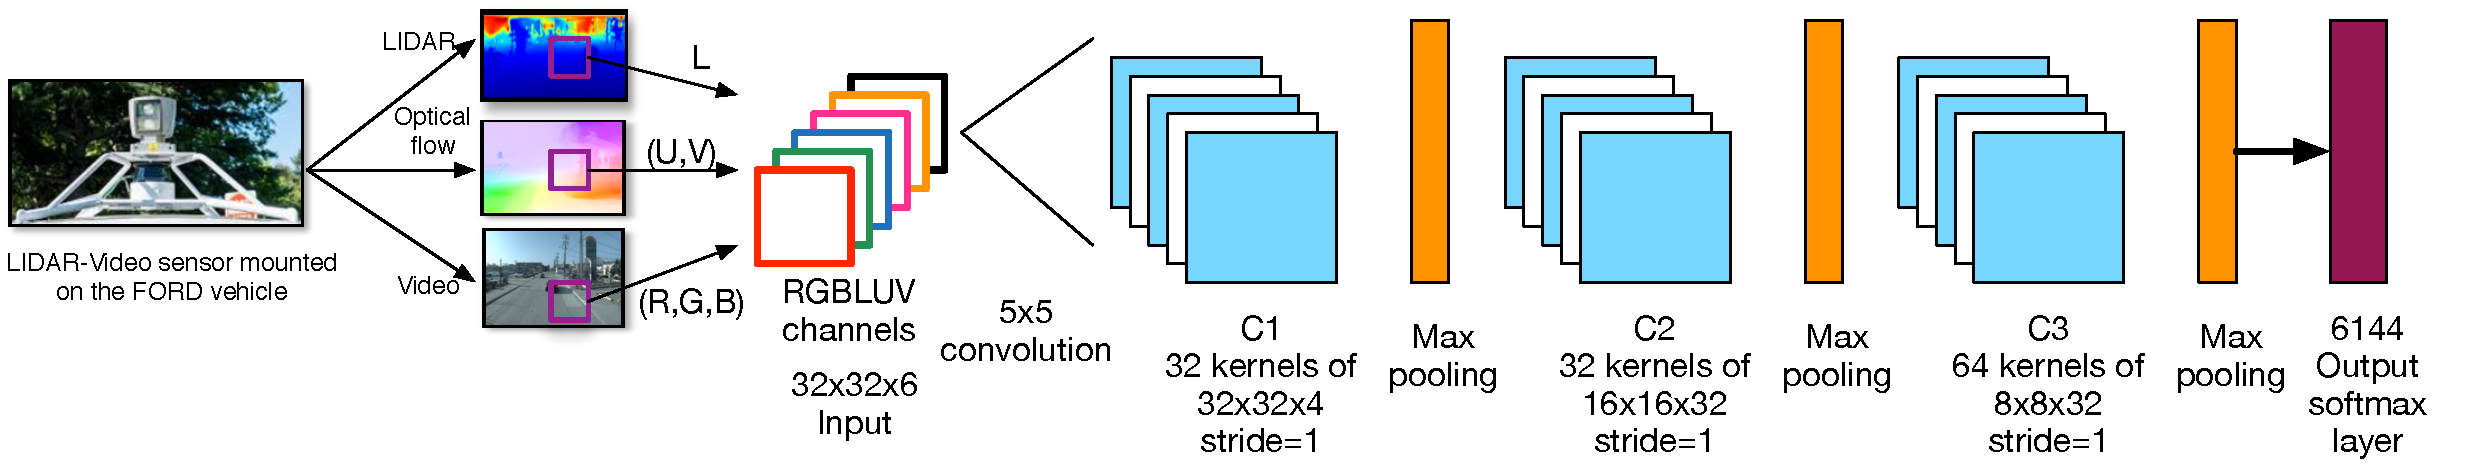
\includegraphics[scale=0.35]{Figures/lidar_dcnn_setup1.pdf}
    \caption{Experimental setup of the LIDAR-Video DCNN}
    \label{fig:Figures_lidar_dcnn_setup1}
\end{figure}

% subsection ford_lidar_video_dataset_and_experimental_setup (end)

\subsection{Preprocessing} % (fold)
\label{sub:preprocessing}
%image of LVF data with channels, patches and images(frames) denoted.
At each video frame timestep, the inputs to our model consisted of C-channels of data with C ranging from 3-6 channels. Channels consisted of inputs that included greyscale and (R,G,B)-video channels, horizontal and vertical components of optical flow computed from two consecutive frames and Lidar depth information. Each channel was cropped to a uniform 800x??? pixels. Each time step has an 800 x ??? x C array of integer values.

These arrays were subdivided into p x p x C patches at a prescribed stride. For any experiment we can denote the preprocessing parameters 
\begin{itemize}
\item R,G,B --- Frame color channels.
\item U,V --- optical flow channels.
\item L --- lidar depth channel.
\item C --- number of input channels.
\item p --- patch size.
\item s --- stride.
\end{itemize}  

For a given frame of size 800 x h there are approximately n= (800 x h)/s patches (exact number?). The training and test sets had X and Y frames respectively, therefore the entire data set consists of  N = n x X inputs of the patch-size dimension. 

Preprocessing is repeated O times, where O is the number of offset classes. For this work we used two setups. A 5 class, linearly distributed set of offsets and a 9 class elliptically distributed set of offsets. (see figure x) For each offset class, \textbf{Kishore explain how you generated the data.} 
%figure showing offset classes. 

In order to accurately detect misalignment in the LV sensor data, we've assumed there needs to be a lower bound on the amount of information present in each channel. For this data set, L was the only channel with regions of low information. A preprocess step was to eliminate all patches corresponding to L data with variance <x. This leads to the elimination of the majority of foreground patches in the data set, reducing the size of the training set by \textbf{z pct KISHORE}

% subsection preprocessing (end)

% section problem_statement (end)

\section{Model Description}
\textbf{need to describe the parameters post-processing,classification metric for each patch,a table with common params for the experiments would help,voting scheme}

The model consists of a 4-layer \textbf{?} CNN classifier \textit{see image of network} that estimates the offset between the LV inputs at each time step. For each patch within a timestep, there are O variants with the LVF inputs offset by the predetermined amounts. The CNN outputs to a softmax layer, thereby providing an offset classification value for each patch of the frame. 
% figure of the colored class choices for the 5 class data set
figure x: In the 5 class example we color each patch of the frame with a color corresponding to the predicted class. 

For each frame a simple voting scheme is used to aggregate the patch level offset predictions to frame level predictions. A sample histogram of the patch level predictions is show in figure x.

\subsection{optical flow} \textit{kishore, please discuss the motivation to include dynamics, how we performed it and how we'd need to do it if running in real time. this is where we can point ot proof that it improves prediction.}
Optical flow gives a rough estimate of velocity at each pixel given two consecutive frames. Given a stationary scene, the optical flow between two consecutive frames with small motion depends on the distance of the pixel from the camera. For example, closer the pixel, higher the displacement. We intent to use optical flow obtained from video as a proxy for depth. \cite{Opticalflow_realtime} demonstrated that optical flow can be performed in real-time on FPGA and GPU architectures. In our work, we used the algorithm described in \cite{LiuOpticalFlow} for computing optical flow.

\section{Experiments and Post-processing} % (fold)
\label{sec:experiments_and_post_processing}
\textit{Need a complete list of the experiments run
images to visualize the frame level results
please place any confusion matrices and your comments on what you think the results say.
feel free to suggest any tables or other visuals to include.}

\subsection{5 class tests}
% require a table of the different parameter settings, along with some aggregate measures from the confusion matrices. 
In our initial tests, the linearly distributed set of 5 offsets of the LV data were performed. Table 1 lists the inputs and CNN parameters explored ranked in the order of increasing accuracy \textbf{(define accuracy and other cm metrics), include training vs test error and conf mats if room allows}.  

As can be seen ... 

\subsection{9 class tests}
% require a table of the different parameter settings, along with some aggregate measures from the confusion matrices. 
The subsequent tests were designed to understand whether the simple linear displacement model of the 5-class test could be generalized to a model capable of discriminating multiple directions and displacement magnitude. To achieve this 8 positions were chosen on an ellipse along with it's center \textbf{describe the parabola}. LV was offset in a manner similar to the 5 class test. Nine training and test sets were generated and an identical patch level CNN was constructed differing only in the 9 class softmax output layer. 

Table 2 lists the inputs and CNN parameters explored ranked in the order of increasing accuracy \textbf{(define accuracy and other cm metrics), include training vs test error and conf mats if room allows}.  

 \textbf{Discussion: what results confirmed expectations or surprised us (grey scale). Can we confidently say optical flow improves prediction. }


% section experiments_and_post_processing (end)

\section{Conclusions and Future Work} % (fold)
\label{sec:conclusions_and_future_work}
We did it. We're great.

future: implement a method that doesn't require ground truth and also generalizes easily to a wide array of sensors. Test it on data collected from airborne platforms that are noisier and have more degrees of freedom. 

% section conclusions_and_future_work (end)


\section{references}
populate the papers to be cited in the folder and if possible the bib file


\bibliographystyle{iclr2015}
\bibliography{references}

\end{document}
